%% ----------------------------------------------------------------
%% Thesis.tex -- MAIN FILE (the one that you compile with LaTeX) MAIN REPORT
%% ---------------------------------------------------------------- 

% Set up the document
\documentclass[a4paper, 12pt, twoside]{Thesis}  % Use the "Thesis" style, based on the ECS Thesis style by Steve Gunn
\graphicspath{Figures/}  % Location of the graphics files (set up for graphics to be in PDF format)

% Include any extra LaTeX packages required
\usepackage[square, numbers, comma, sort&compress]{natbib}  % Use the "Natbib" style for the references in the Bibliography\cite{Reference2}
\usepackage{verbatim}  % Needed for the "comment" environment to make LaTeX comments
\usepackage{vector}  % Allows "\bvec{}" and "\buvec{}" for "blackboard" style bold vectors in maths
\usepackage{url}
\hypersetup{urlcolor=blue, colorlinks=true}  % Colours hyperlinks in blue, but this can be distracting if there are many links.

\usepackage{float}
\usepackage{listings}
\usepackage{lscape}
\usepackage{multirow}
%\usepackage{lineno}
%\linenumbers
%% ----------------------------------------------------------------
\begin{document}
\frontmatter      % Begin Roman style (i, ii, iii, iv...) page numbering

% Set up the Title Page
\title  {Using Data Abstraction and Inter-Frame Interpolation for Low Data Rate Communication Between a 3D Camera and VR Headset}
\authors  {\texorpdfstring
            {Adam Melvin}
            {Author Name}
            }
\addresses  {\groupname\\\deptname\\\univname}  % Do not change this here, instead these must be set in the "Thesis.cls" file, please look through it instead
\date       {\today}
\subject    {}
\keywords   {}

\maketitle
%% ----------------------------------------------------------------

\setstretch{1.3}  % It is better to have smaller font and larger line spacing than the other way round

% Define the page headers using the FancyHdr package and set up for one-sided printing
\fancyhead{}  % Clears all page headers and footers
\rhead{\thepage}  % Sets the right side header to show the page number
\lhead{}  % Clears the left side page header

\pagestyle{fancy}  % Finally, use the "fancy" page style to implement the FancyHdr headers


%% ----------------------------------------------------------------

% The Abstract Page
%\addtotoc{Abstract}  % Add the "Abstract" page entry to the Contents
\abstract{
%\addtocontents{toc}{\vspace{1em}}  % Add a gap in the Contents, for aesthetics

The application of Virtual Reality (VR) to telerobotics is a current area of study in industry due to a desire for the increased spacial awareness VR provides. However, attempts to implement such a system using standard teleoperation techniques result in sub-par performance and an uncomfortable experience for the user; the benefits of a VR based system are entirely eliminated. The system proposed by this project incorporates elements of data abstraction and inter-frame interpolation to produce lower latency abstractions of the environment, as opposed to the normal approach of aiming for the presentation of an exact replica. A major challenge in the creation of this system is in the real-time application of data abstraction to a video feed; the solution devised to meet this challenge is detailed in this report.
}

\clearpage  % Abstract ended, start a new page
%% ----------------------------------------------------------------

\pagestyle{fancy}  %The page style headers have been "empty" all this time, now use the "fancy" headers as defined before to bring them back


%% ----------------------------------------------------------------
\lhead{\emph{Contents}}  % Set the left side page header to "Contents"
\tableofcontents  % Write out the Table of Contents

%% ----------------------------------------------------------------
\lhead{\emph{List of Figures}}  % Set the left side page header to "List if Figures"
\listoffigures  % Write out the List of Figures

%% ----------------------------------------------------------------

% The Acknowledgements page, for thanking everyone
\acknowledgements{
%\addtocontents{toc}{\vspace{1em}}  % Add a gap in the Contents, for aesthetics

I would like to thank Klaus-Peter Zauner and all the people who have had to put up with being constantly on camera for their patience. I would also like to thank Tom Darlison for allowing me access to his photographs.

}
\clearpage  % End of the Acknowledgements
%% ----------------------------------------------------------------

%% ----------------------------------------------------------------
\mainmatter	  % Begin normal, numeric (1,2,3...) page numbering
\pagestyle{fancy}  % Return the page headers back to the "fancy" style

% Include the chapters of the thesis, as separate files
% Just uncomment the lines as you write the chapters

\chapter{Introduction}

Lorem ipsum dolor sit amet, consectetur adipiscing elit. Vivamus at pulvinar nisi. Phasellus hendrerit, diam placerat interdum iaculis, mauris justo cursus risus, in viverra purus eros at ligula. Ut metus justo, consequat a tristique posuere, laoreet nec nibh. Etiam et scelerisque mauris. Phasellus vel massa magna. Ut non neque id tortor pharetra bibendum vitae sit amet nisi. Duis nec quam quam, sed euismod justo. Pellentesque eu tellus vitae ante tempus malesuada. Nunc accumsan, quam in congue consequat, lectus lectus dapibus erat, id aliquet urna neque at massa. Nulla facilisi. Morbi ullamcorper eleifend posuere. Donec libero leo, faucibus nec bibendum at, mattis et urna. Proin consectetur, nunc ut imperdiet lobortis, magna neque tincidunt lectus, id iaculis nisi justo id nibh. Pellentesque vel sem in erat vulputate faucibus molestie ut lorem.

\section{A Section}

Quisque tristique urna in lorem laoreet at laoreet quam congue. Donec dolor turpis, blandit non imperdiet aliquet, blandit et felis. In lorem nisi, pretium sit amet vestibulum sed, tempus et sem. Proin non ante turpis. Nulla imperdiet fringilla convallis. Vivamus vel bibendum nisl. Pellentesque justo lectus, molestie vel luctus sed, lobortis in libero. Nulla facilisi. Aliquam erat volutpat. Suspendisse vitae nunc nunc. Sed aliquet est suscipit sapien rhoncus non adipiscing nibh consequat. Aliquam metus urna, faucibus eu vulputate non, luctus eu justo.

\subsection{A Subsection}

Donec urna leo, vulputate vitae porta eu, vehicula blandit libero. Phasellus eget massa et leo condimentum mollis. Nullam molestie, justo at pellentesque vulputate, sapien velit ornare diam, nec gravida lacus augue non diam. Integer mattis lacus id libero ultrices sit amet mollis neque molestie. Integer ut leo eget mi volutpat congue. Vivamus sodales, turpis id venenatis placerat, tellus purus adipiscing magna, eu aliquam nibh dolor id nibh. Pellentesque habitant morbi tristique senectus et netus et malesuada fames ac turpis egestas. Sed cursus convallis quam nec vehicula. Sed vulputate neque eget odio fringilla ac sodales urna feugiat.

\section{Another Section}

Phasellus nisi quam, volutpat non ullamcorper eget, congue fringilla leo. Cras et erat et nibh placerat commodo id ornare est. Nulla facilisi. Aenean pulvinar scelerisque eros eget interdum. Nunc pulvinar magna ut felis varius in hendrerit dolor accumsan. Nunc pellentesque magna quis magna bibendum non laoreet erat tincidunt. Nulla facilisi.

Duis eget massa sem, gravida interdum ipsum. Nulla nunc nisl, hendrerit sit amet commodo vel, varius id tellus. Lorem ipsum dolor sit amet, consectetur adipiscing elit. Nunc ac dolor est. Suspendisse ultrices tincidunt metus eget accumsan. Nullam facilisis, justo vitae convallis sollicitudin, eros augue malesuada metus, nec sagittis diam nibh ut sapien. Duis blandit lectus vitae lorem aliquam nec euismod nisi volutpat. Vestibulum ornare dictum tortor, at faucibus justo tempor non. Nulla facilisi. Cras non massa nunc, eget euismod purus. Nunc metus ipsum, euismod a consectetur vel, hendrerit nec nunc. % Introduction

\chapter{Background}
\lhead{\emph{Background}}
\section{Data Abstraction}

"Data abstraction" is the phrase that will be used in this report to describe the act of reducing an image down to only its most essential elements. It is similar in concept to an artist sketching a scene as opposed to attempting a full drawing, and is comparable to data compression as the aim is also to reduce the file size of the image, however data abstraction takes a very different approach to solving the problem than standard compression algorithms.

Data compression is the storing of information using a more space efficient encoding \cite{compression}. While some information is lost during lossy compression, the aim regardless of the algorithm used is to retain as much of the original information as possible. In contrast, the aim when utilising data abstraction is to discard all the information that is unnecessary to fulfilling the image's purpose. For example, if all that is required of a image is that basic shapes can be identified, then only the information on the boundaries of the shapes is necessary; the rest of the image can be discarded. An implementation of data abstraction can be seen in Figure \ref{fig:abstraction3rdyear}.

%\caption[My figure Title.]{My figure Title. Details how it was made. What is the point? Reproduced from}

\begin{figure}[H]
    \begin{center}
      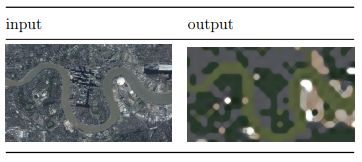
\includegraphics[width=0.6\textwidth]{Figures/abstraction3rdyear.png}
      \caption[Data Abstraction Example]{Data Abstraction Example. This is the abstraction of an aerial photograph of London, reproduced from \cite{abstraction3rdyear}}
      \label{fig:abstraction3rdyear}
    \end{center}
\end{figure}

\section{Sobol Sequences}

Sobol sequences are quasi-random sequences that were introduced to aid in approximating integrals over an S-dimensional unit cube \cite{joe2008constructing}. The aim is to form a sequence $x_i$ in S-dimensional unit cube $I^S$ that approximates
\begin{equation}
    \int_{I^S} f \quad by \quad \lim_{n\to\infty}\frac{1}{n}\sum_{i=1}^{n} f(x_i)
\end{equation}
For this to hold, the points of $x_i$ should be selected so they are evenly spread across $I^S$. This provides a much more even spread of points across the chosen space than can be produced from a pseudo-random number source (Figure \ref{fig:Sobol}). The code used in this project to produce these sequences was created by Leonhard Gr\"unschlo\ss\space \cite{CodeSource} and is presented in Appendix A.

\begin{figure}[H]
    \begin{center}
    \begin{tabular}{ c c }
        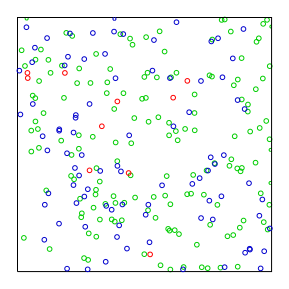
\includegraphics[width=0.33\textwidth]{Figures/Pseudorandom_sequence_2D.png} &
        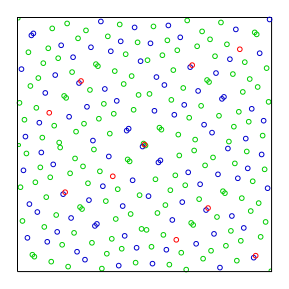
\includegraphics[width=0.33\textwidth]{Figures/Sobol_sequence_2D.png}
    \end{tabular}
    \caption[Comparison of pseudo-random and quasi-random sequences]{Comparison of pseudo-random and quasi-random sequences. 256 points from a pseudo-random generator (left) and 256 points from a Sobol sequence (right), reproduced from \cite{SobolWiki}.}
    \label{fig:Sobol}
    \end{center}
\end{figure}

\section{Computer Vision}

Computer vision is the automatic analysis of images and extraction of the useful information they contain \cite{CVDef}. A raw image is simply a large matrix of colour values, so for a computer to take action based on the contents of an image it must be able to recognise features using analysis of this data. Doing so involves many different techniques such as statistical pattern classification and geometric modelling \cite{ballard1982computer}. All computer vision methods in this project are implemented using the OpenCV libraries, and the example programs provided with them used as starting points for development \cite{OpenCV}.

\subsection{Edge Detection}
When attempting to recognise the features of an image, knowing the locations of the edges of objects within the scene is often very useful. An edge is defined as a significant local change in intensity, usually due to a discontinuity in either the intensity or its first derivative \cite{jain1995machine}. There are many algorithms available that will detect the edges of an image from the locations of these discontinuities. When the most popular algorithms (Laplacian of Gaussian, Robert, Prewitt, Sobel, and Canny) are compared, the most effective in almost all scenarios is Canny edge detection \cite{maini2009study}, therefore this is the algorithm utilised in this project. Canny edge detection \cite{canny1986computational} (Figure \ref{fig:canny1}), and can be divided into 4 stages:
\begin{enumerate}
    \item Reduce noise using a Gaussian filter
    \item Find the intensity gradient of the image by taking the first derivative in the horizontal and vertical directions.
    \item Remove from the gradient map any pixel that is not a local maximum, reducing the edges down to their minimum thickness.
    \item Remove any edge that either has an intensity gradient lower than a lower threshold value or not connected to pixels with a value larger than an upper threshold value (hysteresis thresholding).
\end{enumerate}

\begin{figure}[H]
    \begin{center}
      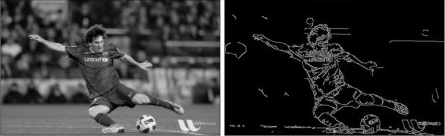
\includegraphics[width=0.9\textwidth]{Figures/canny2.png}
      \caption[Canny Edge Detection Example]{Canny Edge Detection Example. Simple edge detection program applied to a fairly detailed photo of Messi, to demonstrate its effectiveness even with more complex images. Figure taken from an OpenCV Canny tutorial \cite{Canny1Source}.}
      \label{fig:canny1}
    \end{center}
\end{figure}

\subsection{Flood Fill}

Flood fill algorithms determine the area connected to a given cell (the seed point) in a multi-dimensional array that have similar intensity values for the purpose of filling them with a chosen colour \cite{FloodFill}. This is a technique that is not only useful in image processing, but also for many other fields such as in passive acoustic monitoring where finding the area connected to a given node can be useful as part of tracking in 4D space (x,y,z,time) \cite{nosal2008flood}. A demonstration of flood fill has been presented in Figure \ref{fig:EgFloodFill}.

\begin{figure}[H]
    \begin{center}
    \begin{tabular}{ c c }
        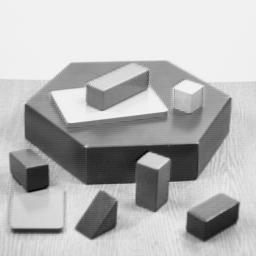
\includegraphics[width=0.35\textwidth]{Figures/blox.jpg} &
        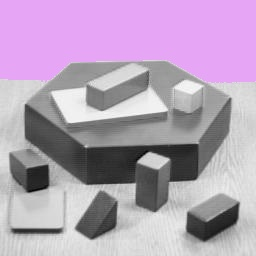
\includegraphics[width=0.35\textwidth]{Figures/bloxFilled.jpg}
    \end{tabular}
    \caption[Example of Flood Fill]{Example of Flood Fill. The original image (left) was provided by OpenCV. The right image is the result of flood filling from the top left corner, filling the lighter space at the back of the scene.}
    \label{fig:EgFloodFill}
    \end{center}
\end{figure} % Background Theory 

\chapter{Progress in Data Abstraction}
\lhead{\emph{Progress in Data Abstraction}}

In this implementation of data abstraction, the aim is to reduce images down to only the boundaries of the objects in the scene and then fill the spaces between theses boundaries with block colours based on the original image. Therefore the general process of the design is:
\begin{enumerate}
    \item Use edge detection on the image, presenting the boundaries of the scene as white lines and the rest as black. 
    \item Divide up the original image into sections that can reasonably be averaged into a single colour, defined by the boundaries produced by the edge detection or otherwise.
    \item Find the average colours (or reasonable alternatives) for these sections.
    \item Flood fill the spaces in the edge detection output with the average colours of the original image.
\end{enumerate}
While this section will be presented in the context of the entire process occurring on a single computer (as this was the testing platform), when incorporated into the final system points 1-3 will be done using the raspberry pi on the rover and point 4 will be done on the computer. This allows for much smaller data packets to be sent over a wireless connection (wifi), due to being able to send the colour information for entire sections of the image as a single colour value.

\section{Edge Detection}

Canny edge detection was implemented using the Canny function provided by OpenCV. The sequence of processes implemented to support the algorithm in producing high quality edges are shown in Figure \ref{fig:CannyProc}. 

\begin{figure}[H]
    \begin{center}
    \begin{tabular}{ c c c }
        (1) & (2) & (3) \\
        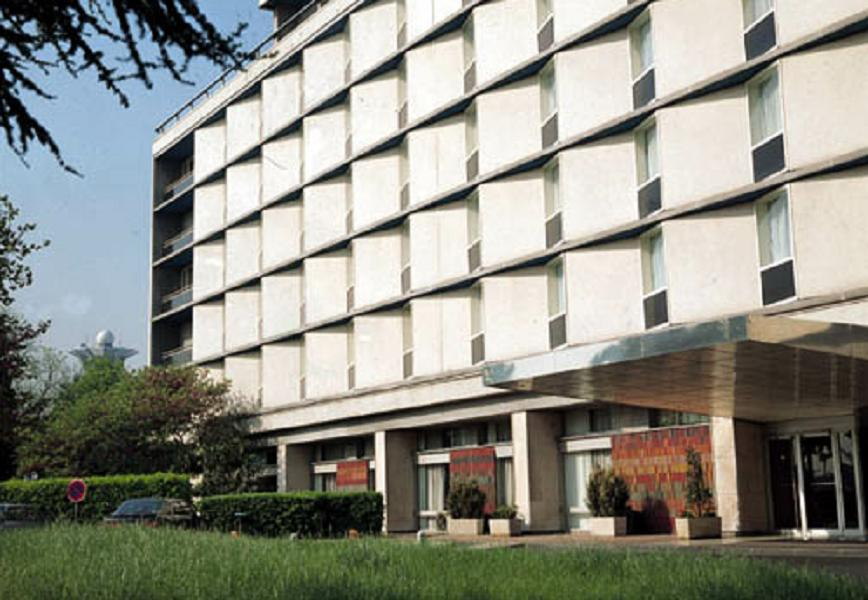
\includegraphics[width=0.31\textwidth]{Figures/building.jpg} &
        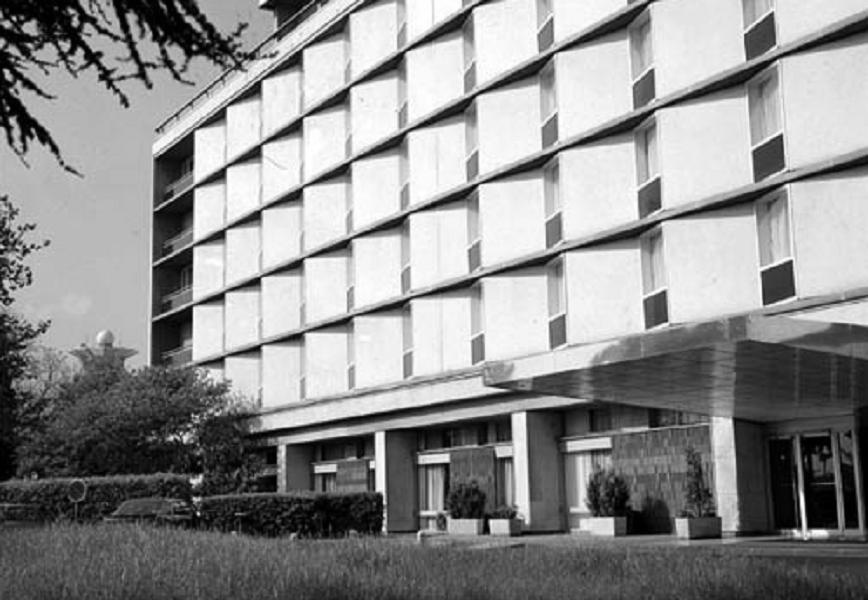
\includegraphics[width=0.31\textwidth]{Figures/buildGray.jpg} &
        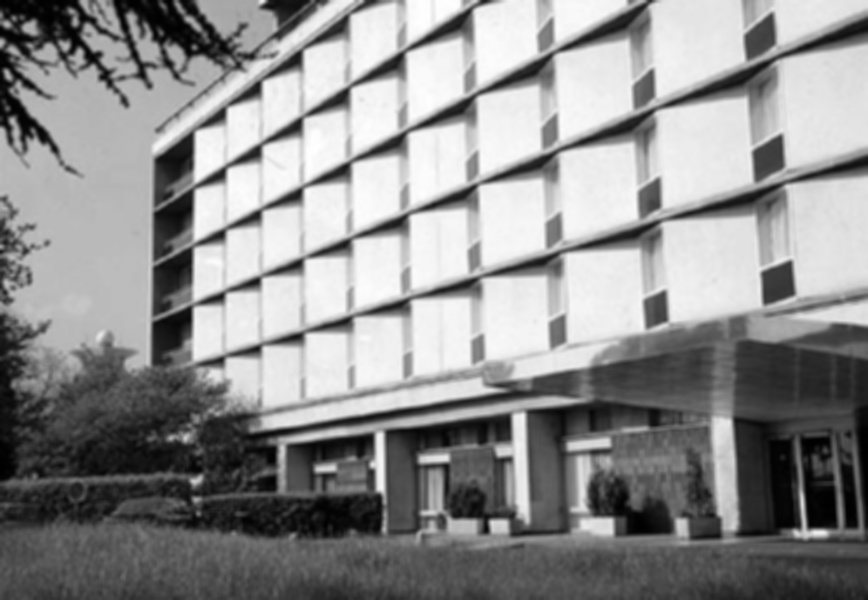
\includegraphics[width=0.31\textwidth]{Figures/buildBlur.jpg}
    \end{tabular}
    \begin{tabular}{ c c }
        (4) & (5) \\
        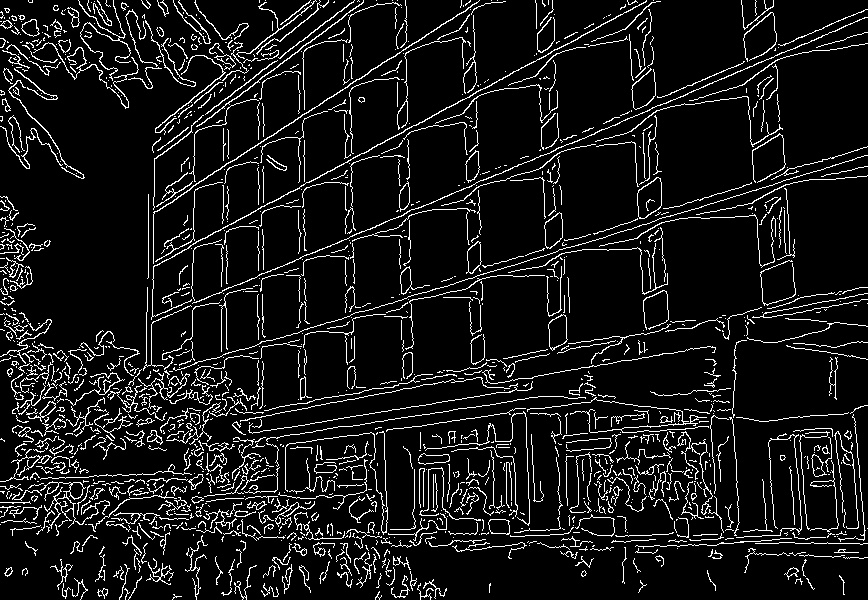
\includegraphics[width=0.31\textwidth]{Figures/buildCanny.jpg} &
        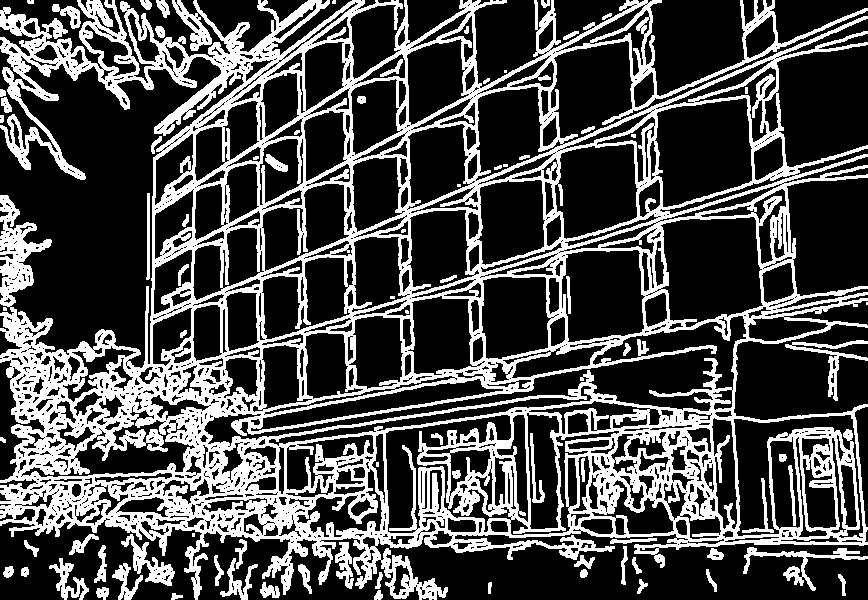
\includegraphics[width=0.31\textwidth]{Figures/buildDilated.jpg}
    \end{tabular}
    \caption[Process of Edge Detection]{(1) the original image, provided by OpenCV, (2) post grayscaling, (3) post blurring, (4) post edge detection, and (5) post dilation.}
    \label{fig:CannyProc}
    \end{center}
\end{figure}

The image is first made grayscale, as Canny detects large changes in light intensity and not colour. The image is then blurred to remove any unnecessary edges and noise that Canny may pick up. The edge detection is used, producing white lines representing the edges on a black background (the details of parameter experimentation with Canny and the previous blurring are presented in Appendix B). The output of the edge detection is finally dilated to make the lines thicker and bridge the gaps between the lines that are very close together. This is done to make the image more cartoon-like and more generally aesthetically pleasing, reduce the number of lines produced by areas that are dense with detail such as hair and foliage (an example of this detail density can be seen in the bush in Figure \ref{fig:Blur}), and to bridge the gaps between lines that are close together, increasing the likelihood of defined shapes being created that can be easily flood filled later.

\section{Flood filling}

Flood filling was chosen as the method for applying colour to the Canny output image, as it is the most efficient way to fill spaces of unknown size and shape that are defined by high contrast boundaries; using it makes dividing up the image into sections unnecessary. To use the OpenCV flood fill function you must provide a seed point to start flooding from, a colour to fill with, and parameters for the filling itself (unchanged from the defaults provided by the OpenCV documentation \cite{opencvffilldemo}).

\subsection{Seed Point}

Finding the points to flood fill from is a challenge, as each image will have a different number of spaces to be filled and the spaces can be anywhere. Three different methods were attempted to solve the problem. The first was an attempt to use OpenCV's contour functionality to provide seed points, however this was unusable due to high resource requirements. The method is detailed in Appendix C.

Although it would by ideal to aim to flood fill from the centre point of each space, it is only necessary if a few specific pixels are being selected to fill from, as each time a line pixel is selected that potential seed point can only be discarded. It is possible to instead iterate through the whole image and flood fill from every pixel found that is not part of a line or an already filled space.

This method is more effective at filling every space than the previous, and is also less resource intensive. However, if presented with a complicated environment with many spaces to flood fill, it must fill every single one, therefore leading to unacceptable drops in frame rate.

The most simple solution to the performance issues caused by allowing the number of times flood fill is used per image to vary would be to set a maximum. However, if this is done the seed points can no longer be selected by iterating through the whole image, as the presence of many small spaces at the top of an image would lead to larger, more important spaces not being filled at the bottom. The solution is to select a set number of points quasi-randomly across the image using Sobol sequencing. Although a certain number of points will land on lines and therefore not be used, if there are enough points then all the important spaces are filled without serious impact on performance. Also, with this method performance is not affected by the complexity of the image, however more complicated images will be processed with many of the more dense areas unfilled (Figure \ref{fig:BrutevsSobol}). For these reasons, the seed points are selected using this method in the current build.

\begin{figure}[H]
    \begin{center}
    \begin{tabular}{ c c }
        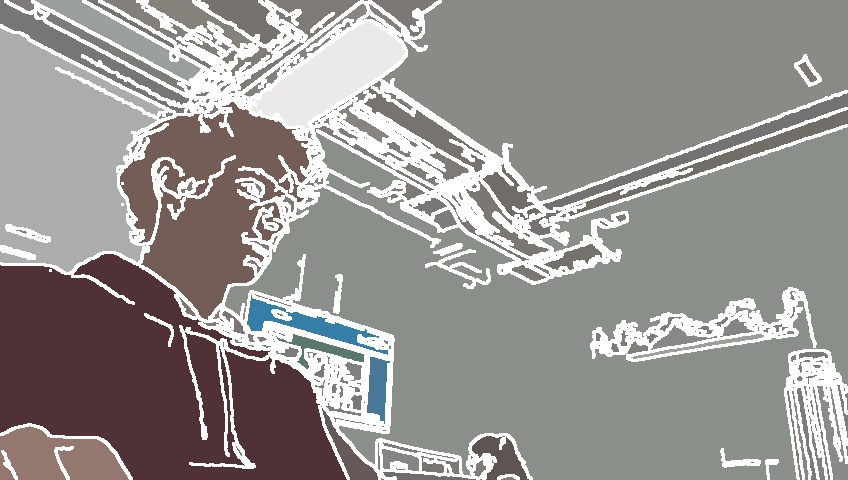
\includegraphics[width=0.45\textwidth]{Figures/Brute.jpg} &
        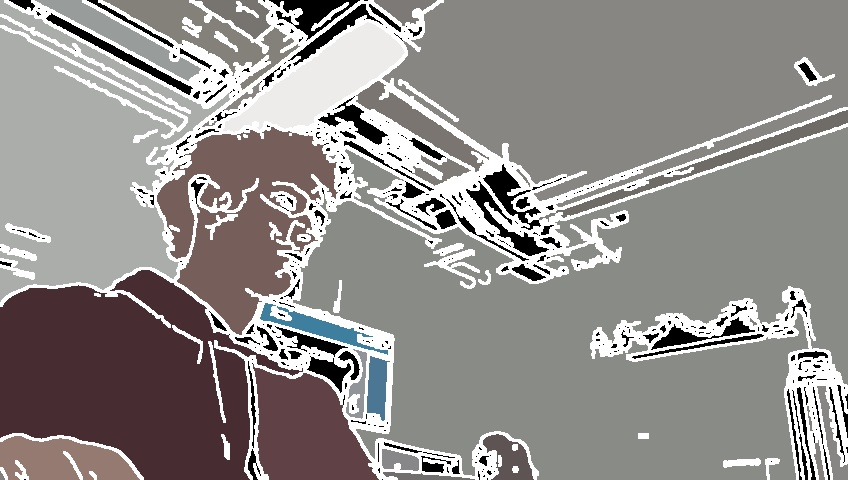
\includegraphics[width=0.45\textwidth]{Figures/Sobol.jpg}
    \end{tabular}
    \caption[Comparison of brute force and Sobol seed point generation]{Comparison of brute force and Sobol seed point generation. It can be clearly seen that the brute force method (left) accurately fills every space in the image, whereas using Sobol results in many unfilled spaces. However, Sobol is higher performance with a frame rate of 17.14fps, compared to 8.57fps using brute force.}
    \label{fig:BrutevsSobol}
    \end{center}
\end{figure}

\subsection{Fill Colour}

Three different methods were considered for finding the colours that the Canny output should be flood filled with. All three methods are valid solutions, but present different ratios between accuracy and resource requirements.

While filling the abstracted image with the average colours present within the input is preferable, it is not essential to the project; provided that the objects in the scene are still recognisable, they don't have to be exactly the right colour. For this reason it would be acceptable to not find the average colour of the area being flood filled at all, and instead simply use the colour of the seed point. This is a very fast method, however produces incredibly inconsistent colours between images. This is because there can be a wide spectrum of colour across a single surface even within the threshold of Canny edge detection, and the Sobol sequence will sample from a different point each time producing spaces that flicker between a wide range of colours.

The consistency of the previous method can be improved substantially with minimal impact on performance by taking an average of the colour within the area of a small circle around the seed point, rather than just the colour of that one point. This significantly improves the consistency between images, however introduces the problem of incorporating pixels from outside the space to be filled. This is due to the quasi-random points often being closer to the edge of the space that they are being flooded from then the radius of the circle. Therefore, the size of the circle must be carefully selected to balance the benefits of increasing size (more consistency when the seed point is further from the edge) and the benefits of decreasing size (more consistency when the seed point is closer to the edge). 

The OpenCV flood fill function provides the ability to fill a blank mask using the boundaries defined by a different image \cite{bradski2008learning}. This makes it possible to create a custom mask with the exact size and shape of the space that is to be filled and use that to find the average colour instead of the predefined circle. This produces the average colour of every space in the image exactly at the expense of adding an extra stage of flood filling before the Canny output itself is filled. The consistency between images for this is the maximum possible based on colour alone (Figure \ref{fig:ColourConsistency}), though inconsistency in the edge detection causes certain spaces to combine and divide constantly, leading to a small amount of colour inconsistency to remain regardless. This method has a noticeable impact on performance, though within acceptable bounds, leading this to be the chosen method for the current build. Examples of the results produced by the final build can be seen in Appendix D.

\begin{figure}[H]
    \begin{center}
      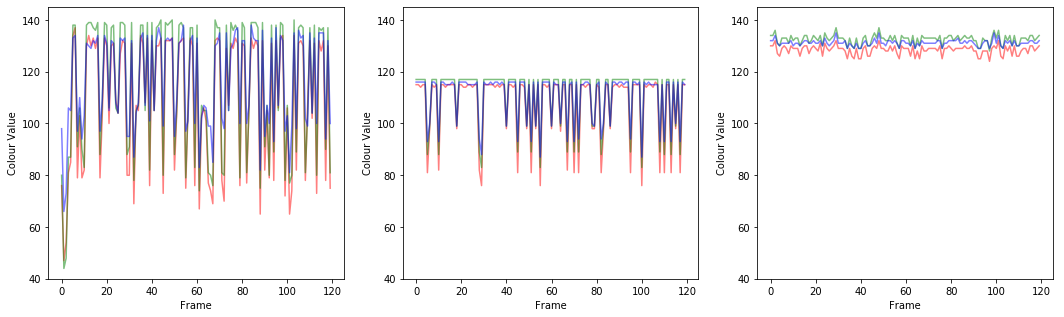
\includegraphics[width=1\textwidth]{Figures/ColourConsistency.png}
      \caption[Comparison of Colour Averaging Methods]{Comparison of Colour Averaging Methods. These are RGB values over time produced by flood filling an example area using the seed point colour (left), circle average (middle), and flood fill average (right). The increase in consistency from left to right is very apparent.}
      \label{fig:ColourConsistency}
    \end{center}
\end{figure} % Experimental Setup

\chapter{Plan for Remaining Work}
\lhead{\emph{Plan for Remaining Work}}

When building a system of this scale, great care must be taken to thoroughly test each stage both individually and in the context of the full system. For this reason, the general approach when organising my time was to work from the start point of the process (the hardware of the rover and the data abstraction it uses), making my way through each stage and combining it with the last to create larger subsections of the system. This also allows for better risk management; if a stage does not function as intended to the extent that the project cannot be completed, the work already done would still function as its own smaller system. A gantt chart providing the details of this approach, both going forward and its results, can be found in Appendix E.

A break down of how the budget has been used so far has been presented in Appendix F. The total budget spent is \pounds124.97, leaving \pounds25.03 spare to be used in the event of hardware failure. Also in Appendix F is a full risk assessment for the project going forward, necessary due to the high risk presented by projects of this scale. % Experiment 1

%\input{Chapters/Chapter5} % Experiment 2

%\input{Chapters/Chapter6} % Results and Discussion

%\input{Chapters/Chapter7} % Conclusion

%% ----------------------------------------------------------------
% Now begin the Appendices, including them as separate files

\addtocontents{toc}{\vspace{2em}} % Add a gap in the Contents, for aesthetics

\appendix % Cue to tell LaTeX that the following 'chapters' are Appendices

\chapter{Sobol Sequence Implementation}
\lhead{\emph{Sobol Sequence Implementation}}

\lstinputlisting[language=C++,caption={sobol.h},label=selection-sort]{Code/sobol.h}
\lstinputlisting[language=C++,caption={sobol.cpp},label=selection-sort]{Code/sobol.cpp}	% Appendix Title

\chapter{Edge Detection Experimentation}
\lhead{\emph{Edge Detection Experimentation}}

The effect of changing the size of the blur kernel was tested (Figure \ref{fig:Blur}), and it was determined that the size of the kernel has a slight effect on both the noise and edge accuracy; reducing the size makes the edges more accurate to the original at the expense of more noise, whereas increasing the size results in less noise but also less accurate edges.

\begin{figure}[H]
    \begin{center}
    \begin{tabular}{ c c c }
        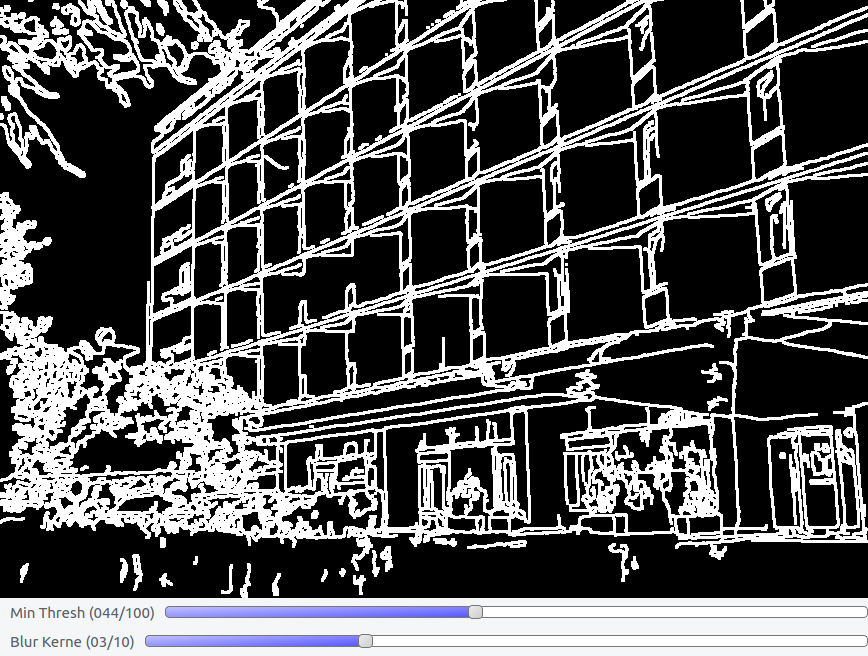
\includegraphics[width=0.31\textwidth]{Figures/Blur1.png} &
        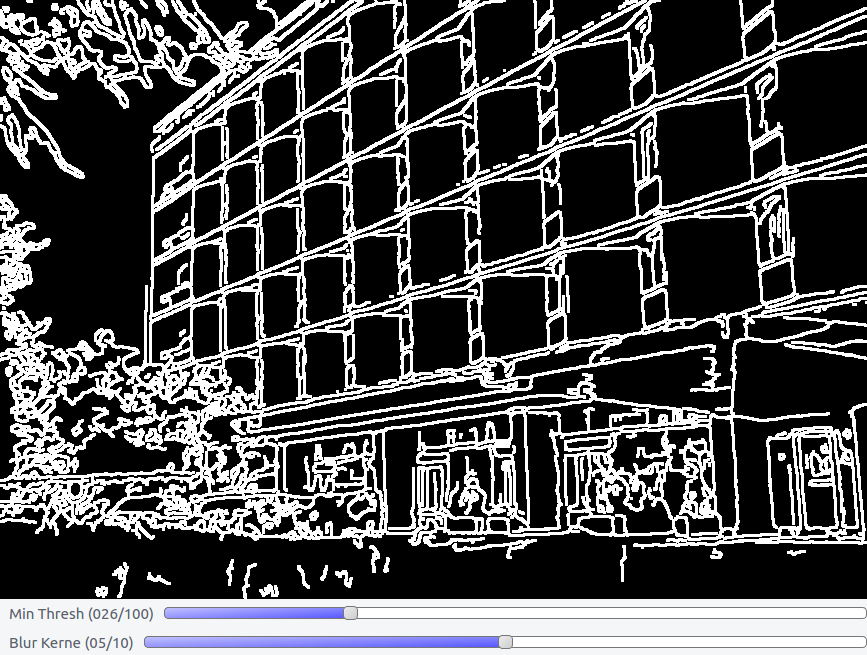
\includegraphics[width=0.31\textwidth]{Figures/Blur2.png} &
        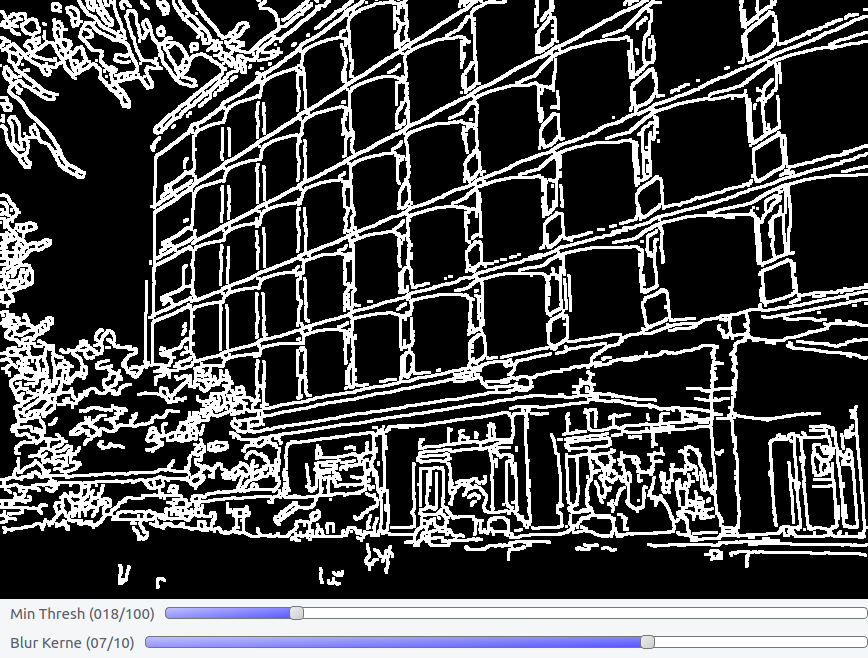
\includegraphics[width=0.31\textwidth]{Figures/Blur3.png}
    \end{tabular}
    \caption[The effect of blurring on edge detection]{The effect of blurring on edge detection. From left to right the size of the square blur kernel is increasing through 3, 5, and 7, and the lower canny threshold is decreasing through 44, 26, and 18 (the threshold change was for the purpose of presenting the best case ratio of detail to noise for each image). This figure shows the minor decrease in noise as the blur kernel increases in size, but also the minor decrease in edge accuracy; this can be seen most clearly in the bush in the bottom right of the frame for noise, and the panels on the upper right of the building for edge accuracy}
    \label{fig:Blur}
    \end{center}
\end{figure}

The edge detection function itself has 3 parameters- low threshold, high threshold, and kernel size. The kernel was set to 3x3 and the high threshold set to 3 times the low threshold by the recommendation of the OpenCV documentation \cite{cannyedgedetector}. From there the effect of changing the low threshold was tested (Figure \ref{fig:Thresh}). Increasing the threshold increased the level of detail at the expense of also increasing the noise. However, it was discerned that different situations can call for drastically different thresholds, therefore necessitating the ability to change the threshold at runtime from within the Unreal 4 environment.

\begin{figure}[H]
    \begin{center}
    \begin{tabular}{ c c }
        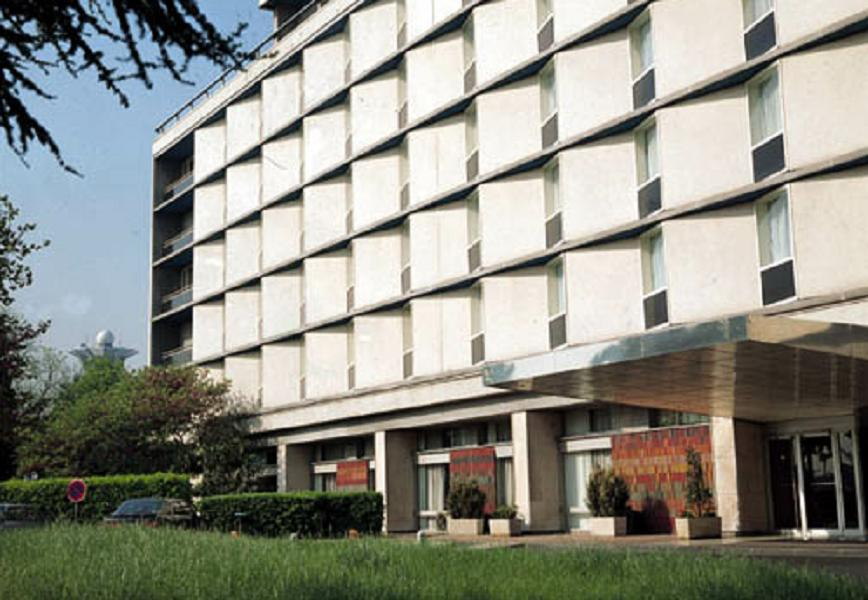
\includegraphics[width=0.405\textwidth]{Figures/building.jpg} &
        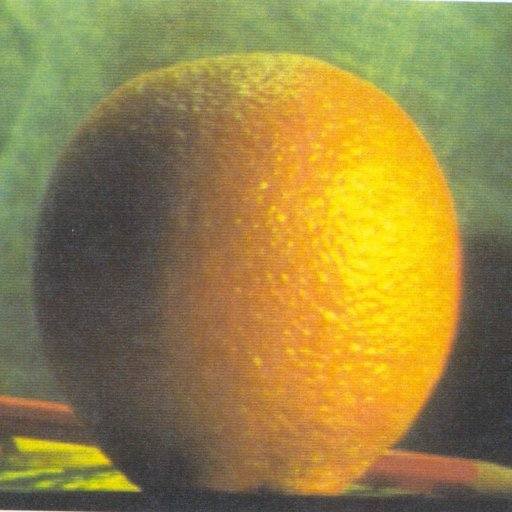
\includegraphics[width=0.28\textwidth]{Figures/orange.jpg} \\
        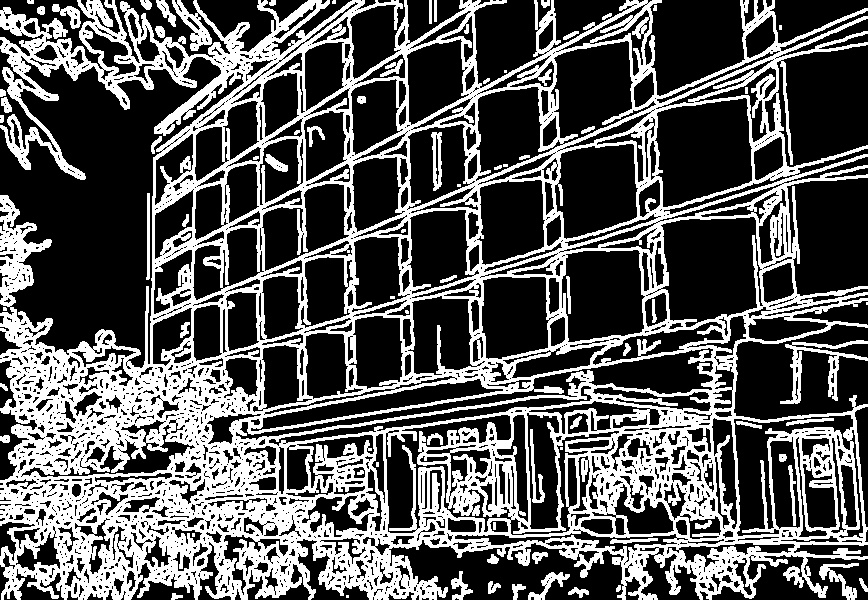
\includegraphics[width=0.405\textwidth]{Figures/buildThresh15.jpg} &
        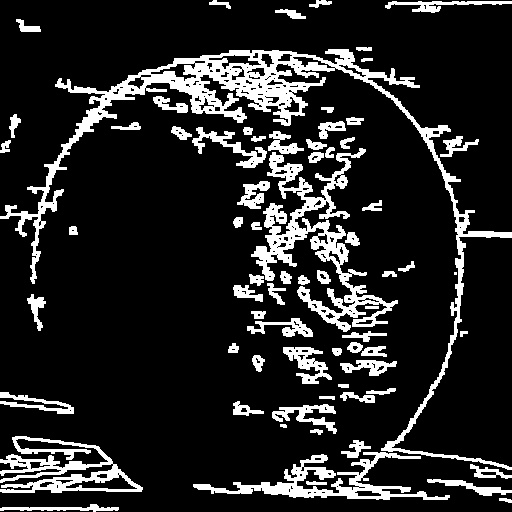
\includegraphics[width=0.28\textwidth]{Figures/orangeThresh15.jpg} \\
        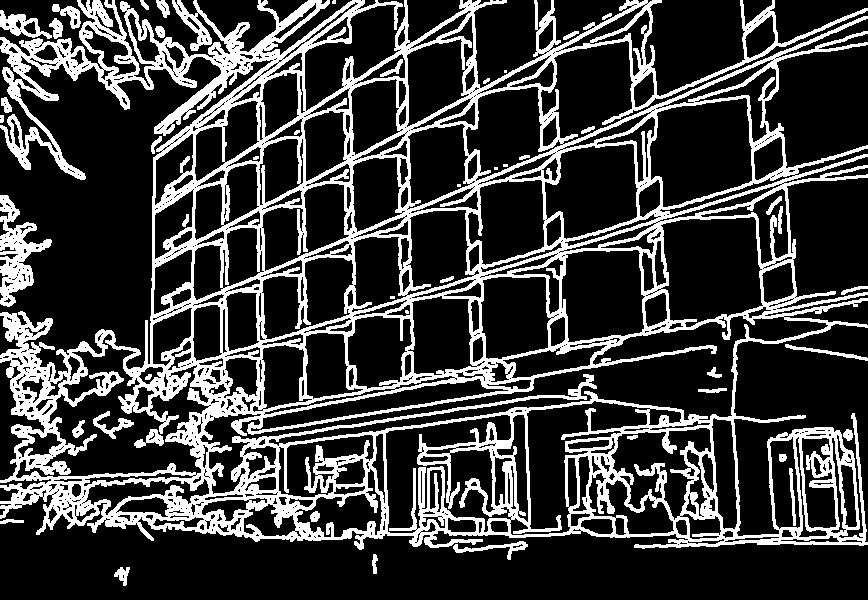
\includegraphics[width=0.405\textwidth]{Figures/buildThresh30.jpg} &
        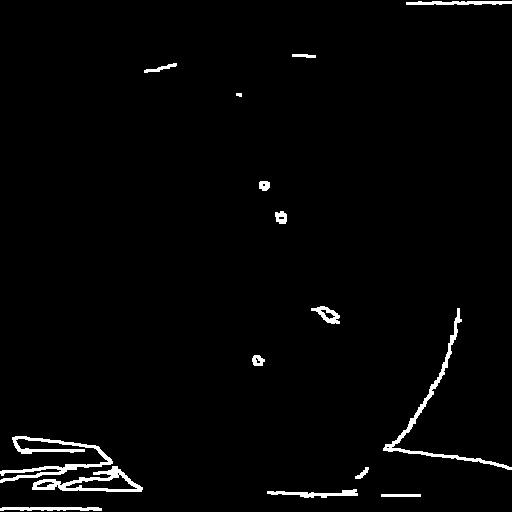
\includegraphics[width=0.28\textwidth]{Figures/orangeThresh30.jpg} \\
        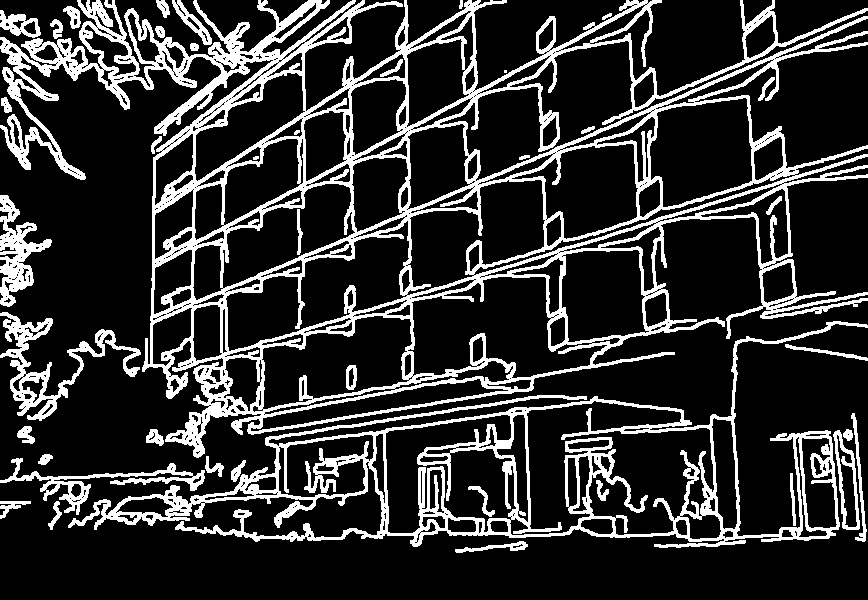
\includegraphics[width=0.405\textwidth]{Figures/buildThresh45.jpg} &
        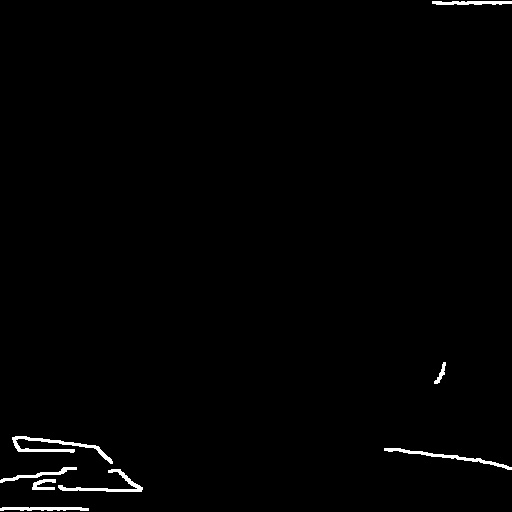
\includegraphics[width=0.28\textwidth]{Figures/orangeThresh45.jpg}
    \end{tabular}
    \caption[The effect of changing Canny threshold values]{The effect of changing Canny threshold values. From top to bottom, presented are images provided by OpenCV, then those images edge detected with low thresholds of 15, 30, and 45. The blur kernel is always 5x5 and the high threshold 3 times the low threshold. It can be seen that the best threshold for the building is 30, whereas the best for the orange is 15. This proves the necessity of being able to change the threshold at run-time to account for different situations.}
    \label{fig:Thresh}
    \end{center}
\end{figure}
 % Appendix Title

\chapter{Contour Based Seed Point Location}
\lhead{\emph{Contour Based Seed Point Location}}

The ideal place to aim to flood fill a space from would be the centre point of the space. OpenCV provides the functionality to take the Canny output image (a matrix of colour values) and convert it into a set of contours. Contours are line objects stored in a hierarchical structure and have functions that can provide the centre point of each contour. Although the centre points of the contours will not map exactly to the centre points of the space, they are close enough approximations to flood fill from (Figure \ref{fig:ContourCentres}).

Unfortunately, due to a combination of the processing time required to convert the lines into contours and the number of contours produced that have no impact on the spaces left to be flood filled, this method is too resource heavy to produce 10 fps on a laptop, therefore is also too resource heavy for use on the raspberry pi.

\begin{figure}[H]
    \begin{center}
    \begin{tabular}{ c c }
        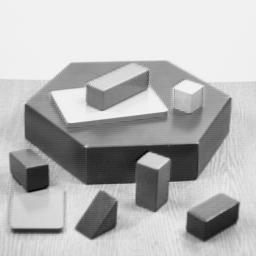
\includegraphics[width=0.31\textwidth]{Figures/blox.jpg} &
        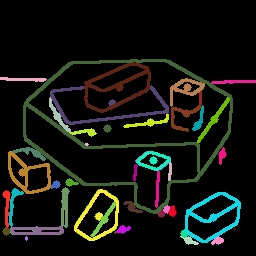
\includegraphics[width=0.31\textwidth]{Figures/ContourCentres.jpg}
    \end{tabular}
    \caption[Demonstration of contour centre point location]{Demonstration of contour centre point location. The original image (provided by OpenCV) on the left has been Canny edge detected, these edges have converted into contours, and the centre points of these contours located. The results of this are displayed on the right, with each contour and its corresponding centre point in a different colour. It can be observed that the centre points provide adequate coverage of the black spaces in the image to be used as seed points for flood filling.}
    \label{fig:ContourCentres}
    \end{center}
\end{figure}
 % Appendix Title

\chapter{Demonstrations of Full Data Abstraction}
\lhead{\emph{Demonstrations of Full Data Abstraction}}

\begin{figure}[h]
    \begin{center}
    \begin{tabular}{ c c }
        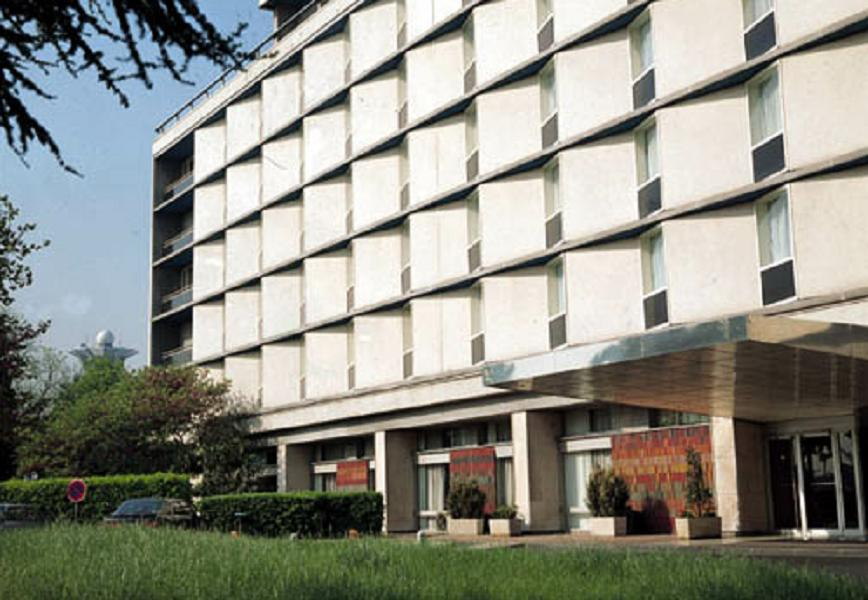
\includegraphics[width=0.45\textwidth]{Figures/building.jpg} &
        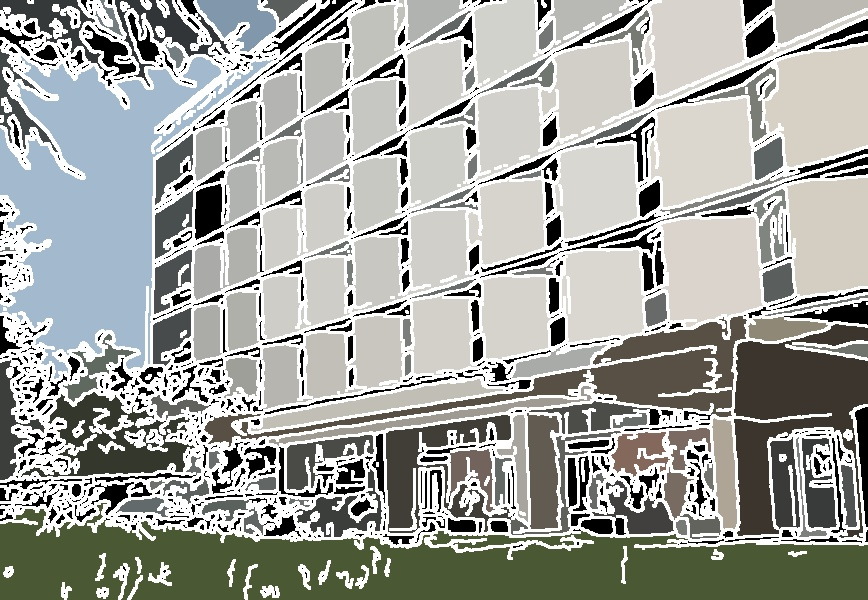
\includegraphics[width=0.45\textwidth]{Figures/Final.jpg} \\
    \end{tabular}
    \caption[Demonstration of full abstraction process]{Demonstration of full abstraction process. The final parameters and methods (of those under discussion) are a blur kernel of 5x5, a low threshold of 25 (for this example), Sobol seed point generation, and averaging via preliminary flood fill. It can be seen that most areas of the image are being effectively edge detected and flood filled with the correct colours; however, some areas are hard to interpret such as around the bushes in the bottom left, and some spaces have been left unfilled such as the panel below the top left corner of the building. These issues are minimal though, therefore leading me to conclude that the process is effective at producing recognisable abstractions of the input images.}
    \label{fig:Final}
    \end{center}
\end{figure}
        
\begin{figure}[h]
    \begin{center}
    \begin{tabular}{ c c }
        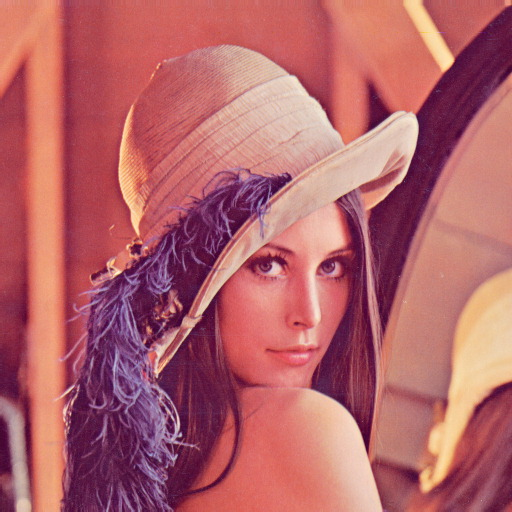
\includegraphics[width=0.45\textwidth]{Figures/lena.jpg} &
        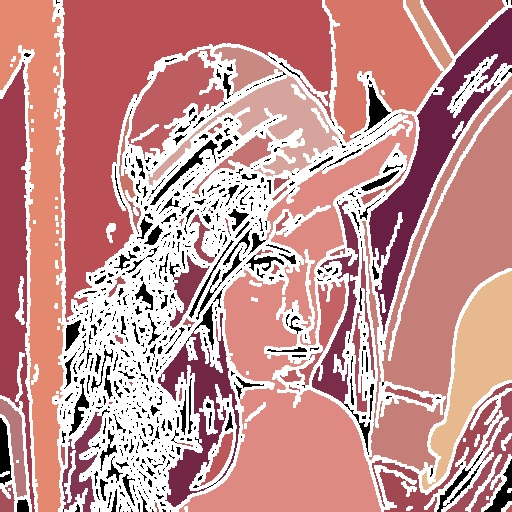
\includegraphics[width=0.45\textwidth]{Figures/lenaDA.jpg} \\
        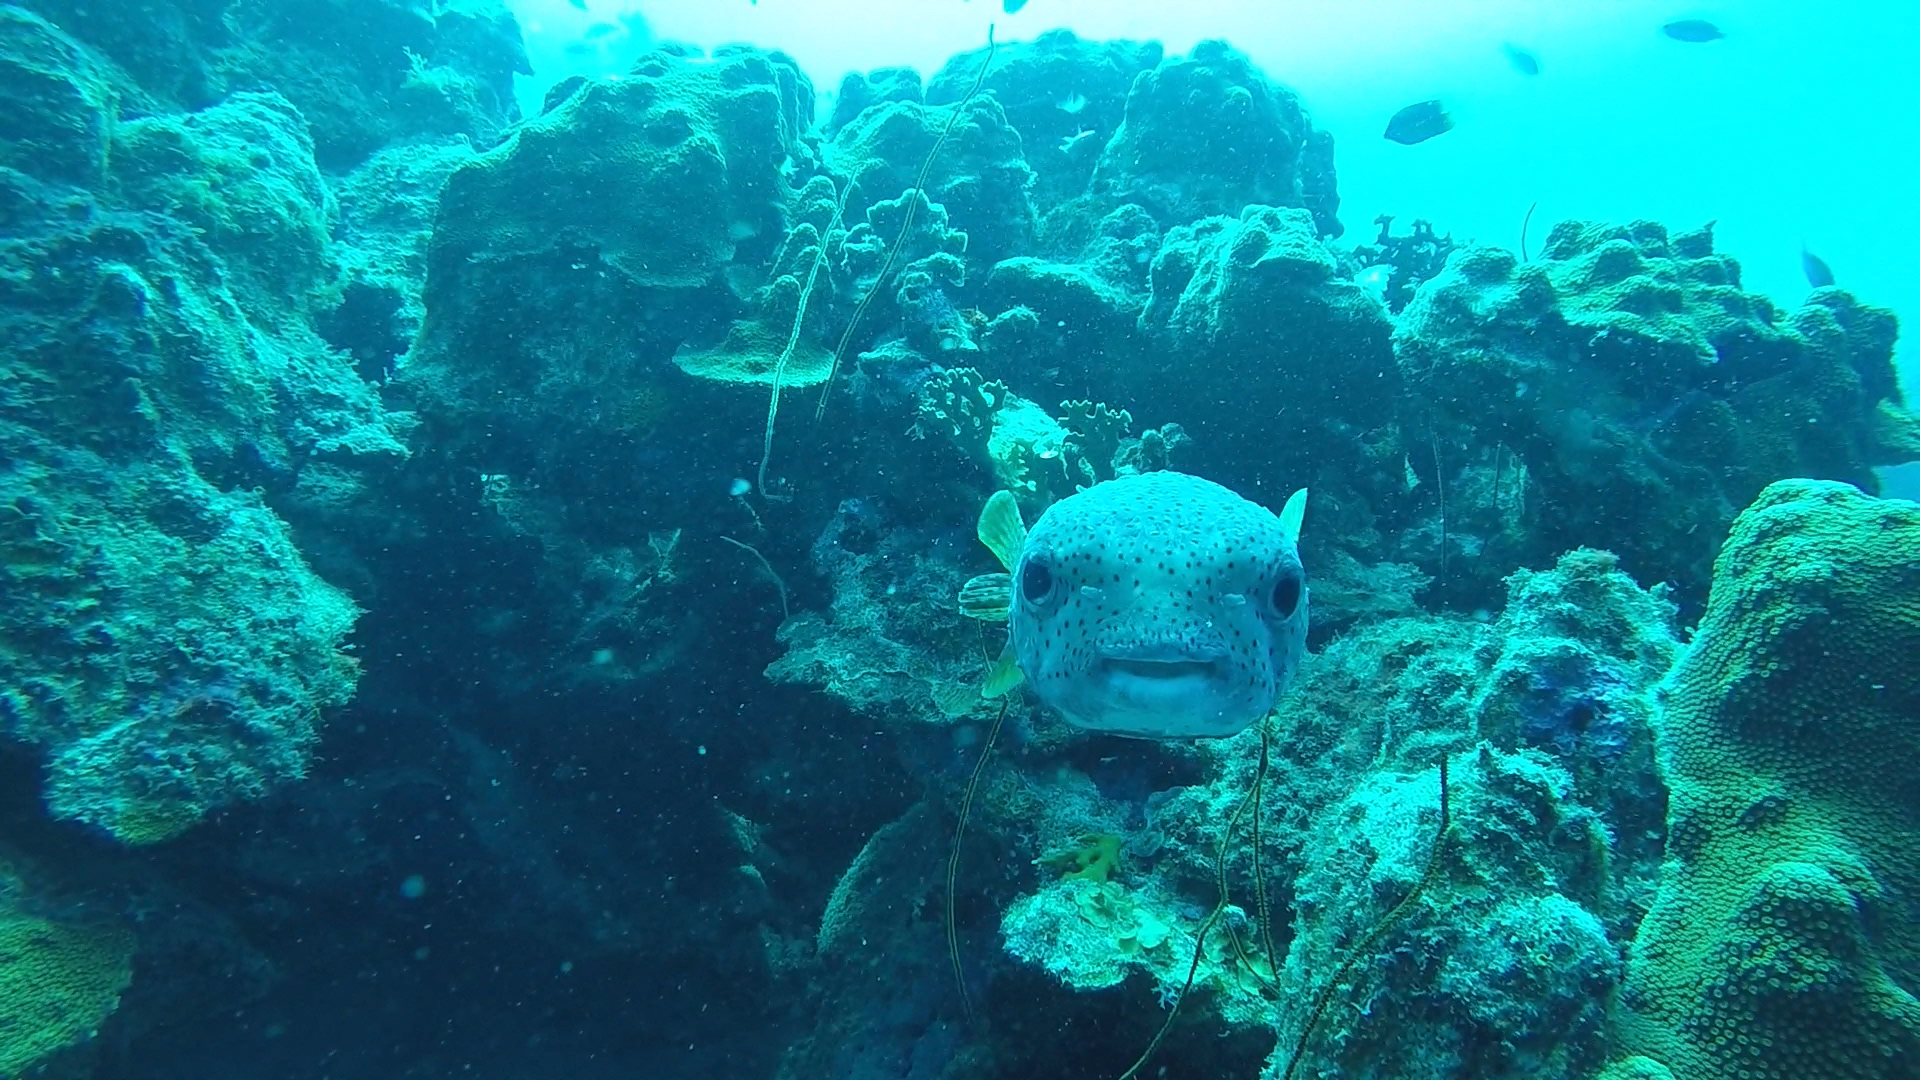
\includegraphics[width=0.45\textwidth]{Figures/pufferfish6.jpg} &
        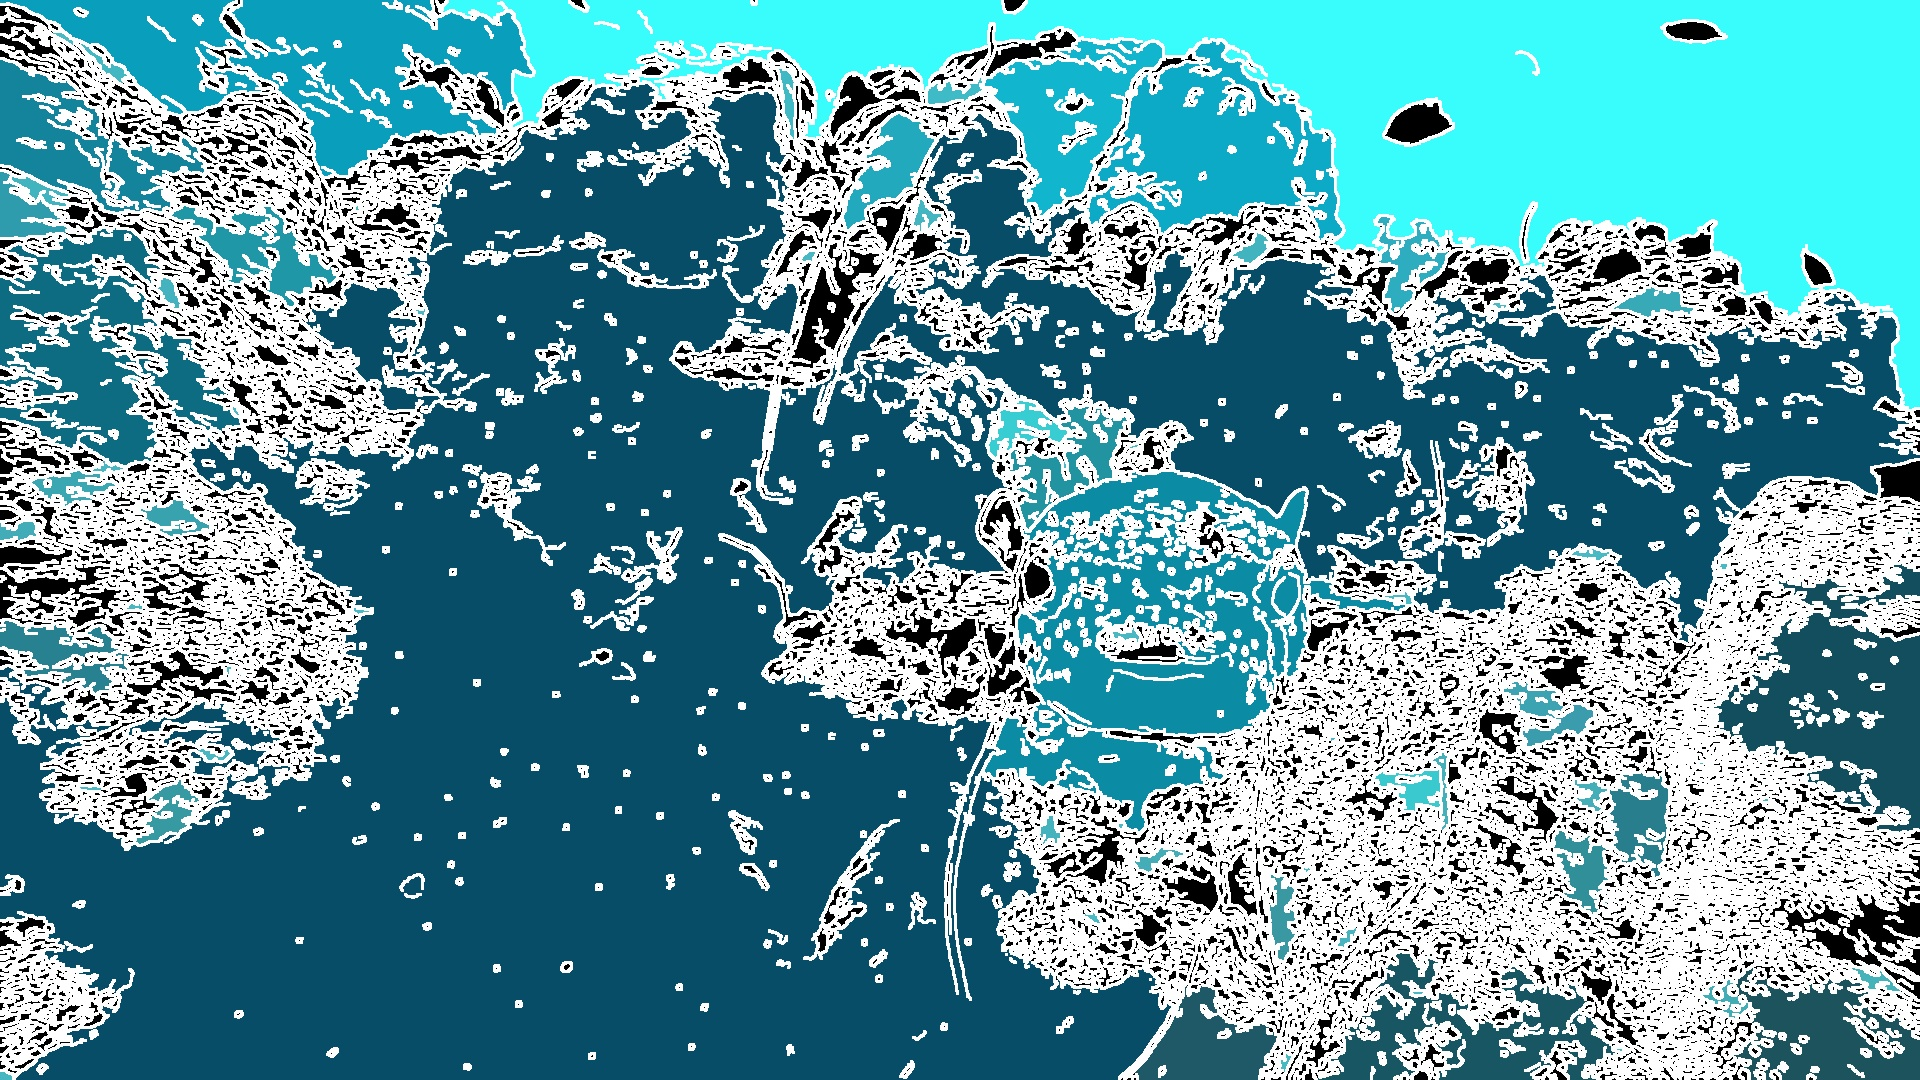
\includegraphics[width=0.45\textwidth]{Figures/pufferfishDA.jpg} \\
        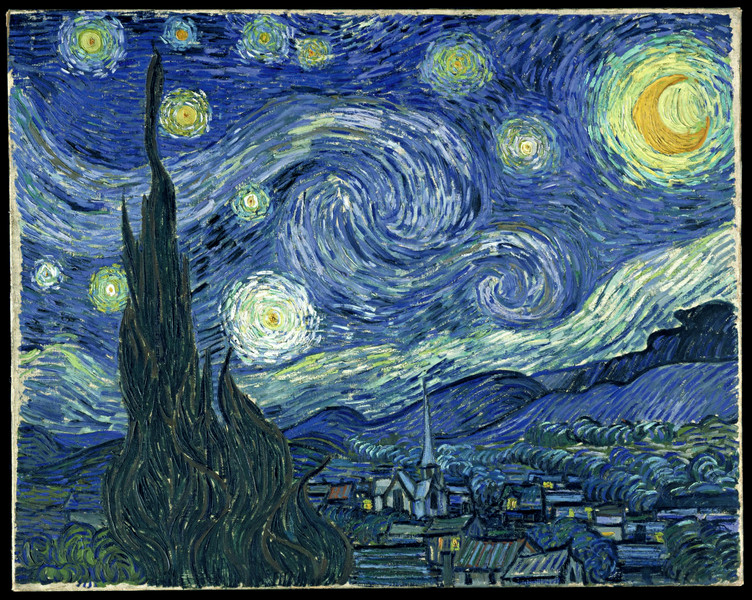
\includegraphics[width=0.45\textwidth]{Figures/starry_night.jpg} &
        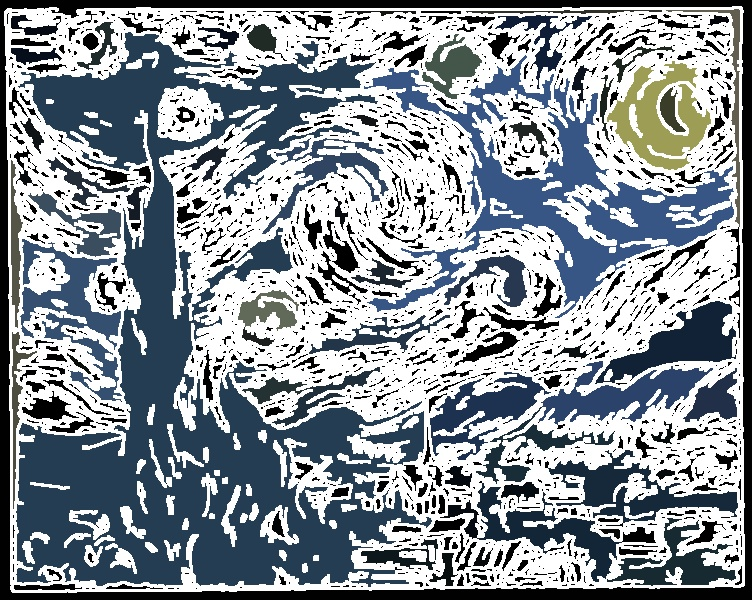
\includegraphics[width=0.45\textwidth]{Figures/starry_nightDA.jpg} 
    \end{tabular}
    \caption[Additional examples of the full abstraction process]{Additional examples of the full abstraction process. The top image (provided by OpenCV) is very simple, so the abstraction gives clean and easily recognisable results. The middle image (provided by fellow student Tom Darlison) was selected due to its limited colour palette and poor focus to test the limits of the process. While the image has mostly filled to a single colour, the pufferfish, rocks, coral, background fish, and open water are all identifiable. The bottom image (provided by OpenCV) was selected due to the extreme number of edges, due to the very clear brush strokes. Once the Canny threshold was turned down considerably, the result was recognisable as Starry Night, though much of the image has been overwhelmed by the edge detection lines. It can be concluded from these tests that the data abstraction process is effective at producing recognisable images, however the difficulty in interpreting the abstracted images is heavily dependant on the focus and complexity of the image.}
    \label{fig:FinalExtras}
    \end{center}
\end{figure} % Appendix Title

\chapter{Gantt Chart}
\lhead{\emph{Gantt Chart}}
\begin{landscape}
\begin{figure}[ht]
    \begin{center}
    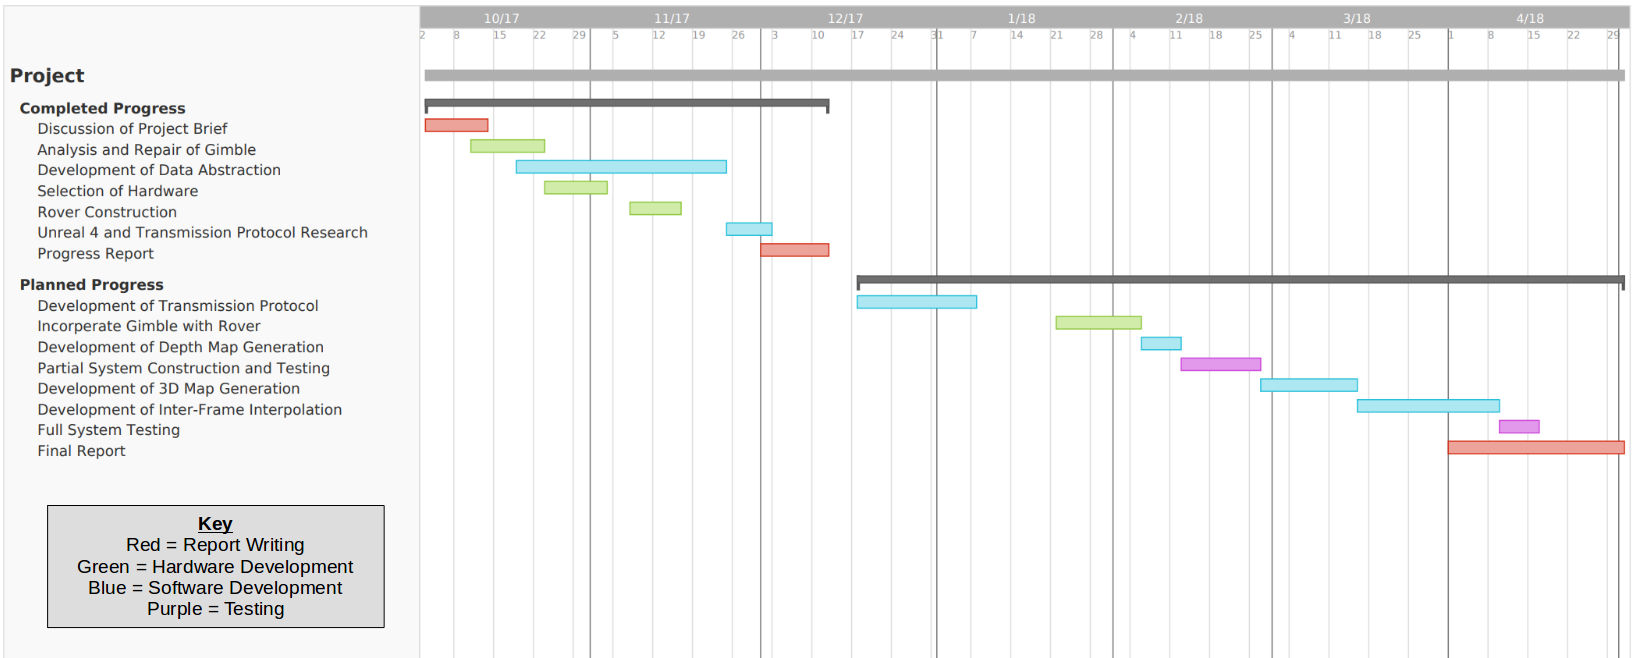
\includegraphics[width=1.5\textwidth]{Figures/ganttfinal.png}
    \label{fig:GanttChart}
    \end{center}
\end{figure}
\end{landscape} % Appendix Title

\chapter{Costing and Risk Assessment}
\lhead{\emph{Costing and Risk Assessment}}

\begin{figure}[H]
    \begin{center}
      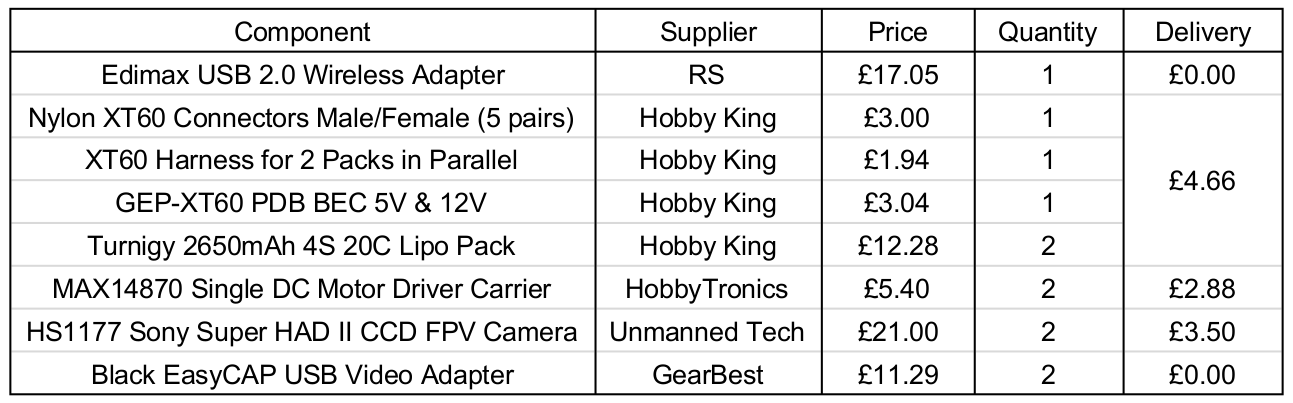
\includegraphics[width=\textwidth]{Figures/Requisitions.png}
      \caption[Hardware Costs List]{Hardware Costs List. This shows the use of budget for this project thus far. Total budget spent = \pounds124.97}
      \label{fig:Costs}
    \end{center}
\end{figure}

\begin{figure}[H]
    \begin{center}
      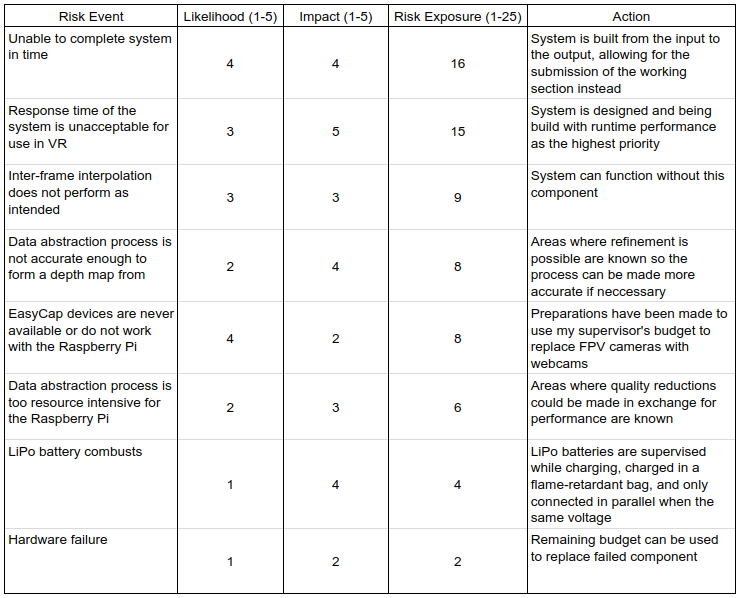
\includegraphics[width=\textwidth]{Figures/RiskAssessment.png}
      \caption[Risk Assessment]{Risk Assessment for the project going forward.}
      \label{fig:Risk}
    \end{center}
\end{figure} % Appendix Title

\addtocontents{toc}{\vspace{2em}}  % Add a gap in the Contents, for aesthetics
\backmatter

%% ----------------------------------------------------------------
\label{Bibliography}
\lhead{\emph{Bibliography}}  % Change the left side page header to "Bibliography"
\bibliographystyle{ieeetr}  % Use the "unsrtnat" BibTeX style for formatting the Bibliography
\bibliography{Bibliography}  % The references (bibliography) information are stored in the file named "Bibliography.bib"
b
\end{document}  % The End
%% ----------------------------------------------------------------